\chapter{Methodology and development process}

\FloatBarrier

\section{Final pipeline and context extraction}

The final method groups released annotations into entity records, selects one deterministic gold centre, extracts capped local relations, inserts them into frozen one-shot templates, generates responses, validates them, and computes paired scores. Figure~\ref{figure:5.1} summarizes these stages. Definitions 2.4–2.9 identify the objects passed between stages.


\begin{figure}[htbp]
\centering
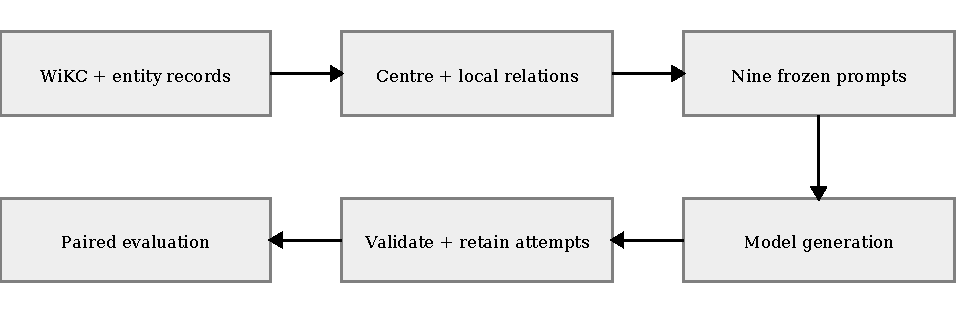
\includegraphics[width=\linewidth]{figures/pipeline.pdf}
\caption{The final generation and evaluation pipeline.}\label{figure:5.1}
\end{figure}

\begingroup
\begin{table}[!htbp]
\setlength{\tabcolsep}{3pt}
\renewcommand{\arraystretch}{1.18}
\fontsize{8.5}{10.5}\selectfont
\renewcommand{\thetable}{5.1}
\renewcommand{\tablename}{Algorithm}
\caption[]{Deterministic oracle context extraction (Definitions 2.5–2.6).}\label{algorithm:5.1}
\begin{tabular}{>{\raggedright\arraybackslash}p{\dimexpr 0.082789\linewidth-2\tabcolsep\relax}>{\raggedright\arraybackslash}p{\dimexpr 0.917211\linewidth-2\tabcolsep\relax}}
\toprule
\textbf{Step} & \textbf{Operation} \\
\midrule
1 & Read all gold identifiers and their annotated depths for entity e. \\
2 & Keep gold classes with no annotated descendant; use all gold classes if this set is empty. \\
3 & Sort by decreasing annotated depth, then ascending identifier string; select c*(e). \\
4 & Find parents, children, and siblings sharing a parent, excluding the centre. Missing graph nodes yield empty lists. \\
5 & Sort each relation list lexicographically and retain its first three identifiers. \\
6 & Render labels for the selected relations; omit the centre label from the context. Keep all gold annotations for evaluation. \\
\bottomrule
\end{tabular}
\end{table}
\endgroup


The omitted centre does not make the context blind to the answer. Its parents and children can strongly constrain the missing class, and the centre is selected using gold annotations. The experiment uses that information to test relevant structure; autonomous deployment would require candidate retrieval without gold access.


\FloatBarrier

\section{Prompt templates and demonstration}

Prompting specifies a task through the text supplied to a language model at inference time. It can describe the required output, provide evidence, and illustrate acceptable behaviour. In-context examples show an input and a desired response without updating model weights. \citet{brown2020} demonstrated the usefulness of this general few-shot setup across language tasks. Here, prompting supplies both the typing instructions and a fixed worked example; no model is fine-tuned on the evaluation entities.


Every final prompt contains one positive demonstration and is therefore one-shot. The external entity is Rod Fergusson (wd:Q18720219), described as a Canadian video game producer, and is outside the 1,000-entity evaluation cohort. The same demonstration entity is used throughout, with condition-specific context and response format. The contrastive style adds an incorrect ranking for that same example; it does not add a second demonstration entity.


Output instructions matter because the model has considerable freedom. The final common instruction requests concise labels, asks for the most specific label first, forbids duplicates and padding, and restricts predictions to evidence-supported types. Graph prompts add a warning that the neighbourhood surrounds an omitted class and is evidence rather than answer options. These instructions address observed tendencies to copy nearby classes, add generic filler, or treat siblings as automatically incompatible.


Prompting remains an empirical design choice. A more elaborate instruction can make the desired behaviour clearer, but it can also alter output length and introduce additional constraints. The study therefore compares fixed templates and retains the generated prompt files. It does not infer that the final wording is optimal. Because the wording was developed using earlier project experience, the full-cohort evaluation is an exploratory assessment of that selected design. A future confirmatory experiment should freeze the templates before opening a new evaluation set.


Chain-of-thought prompting elicits intermediate reasoning before an answer. \citet{wei2022} developed a few-shot formulation in which demonstrations contain reasoning steps as well as final outputs, and evaluated it on reasoning tasks. This motivates an entity-typing prompt that explains why a specific category is supported and how broader categories follow. It does not establish in advance that explanations will improve typing in every model.


The no-graph CoT prompt asks for a brief explanation of the most specific supported type, rejection of unsupported nearby alternatives, and justification of the broader labels and their order. It explicitly limits the evidence to the entity and description. The graph CoT prompt asks the explanation to use parents for semantic scope, compare sibling alternatives, and examine whether child types require unsupported specificity. The output contains an explanation followed by the ordered types list.


This is an adaptation of chain-of-thought prompting to ranked entity typing. “CoT” denotes the explanation-bearing template and demonstration. An explanation is observable output, not a verified account of internal computation: \citet{turpin2023} show that plausible CoT explanations can omit influences on a prediction. Gemini also uses internal thinking under the standard template, so visible explanation and internal reasoning must be distinguished.


Contrastive chain-of-thought prompting adds examples of invalid reasoning alongside valid reasoning. \citet{chia2023} proposed this approach to teach models which mistakes to avoid. The project adapts that principle to entity typing by using a negative demonstration and asking the model to distinguish a supported type from plausible, overly narrow, or incompatible alternatives. The graph version grounds those alternatives in sibling and child relations.


A useful contrast identifies the additional evidence an alternative would require. A class below the centre class may need an attribute absent from the description. A nearby sibling may share a broad parent but describe a different occupation, object, or role. These alternatives can clarify the boundary of a type. However, sibling membership alone does not prove an alternative false. A person can hold several related occupations, and multiple inheritance allows classes to overlap. The final prompt therefore tells the model to reject an alternative only when the evidence warrants rejection.


The contrastive condition is not a reproduction of the original paper’s benchmark or demonstration-construction procedure. It is a task-specific application of learning from correct and incorrect examples. Nor does the presence of sibling labels make every graph prompt formally contrastive: the standard graph prompt also sees siblings, but does not request the same explanation pattern or negative demonstration. These distinctions preserve the meaning of the experimental conditions.


\FloatBarrier

\section{Final prompt conditions and evidence controls}

Table~\ref{table:5.1} defines the nine conditions in Definition 2.9. Standard prompts request a JSON object containing types. CoT and contrastive prompts also request an explanation. Every list is ordered from specific to broad. Appendix C prints all nine complete prompts for framboid, including their actual demonstration text.


\begingroup
\begin{table}[!htbp]
\setlength{\tabcolsep}{3pt}
\renewcommand{\arraystretch}{1.18}
\fontsize{8.5}{10.5}\selectfont
\renewcommand{\thetable}{5.1}
\caption{Nine main conditions and mean Gemini thinking tokens (1,000 completed responses per condition).}\label{table:5.1}
\begin{tabular}{>{\raggedright\arraybackslash}p{\dimexpr 0.261438\linewidth-2\tabcolsep\relax}>{\raggedright\arraybackslash}p{\dimexpr 0.244009\linewidth-2\tabcolsep\relax}>{\raggedright\arraybackslash}p{\dimexpr 0.309368\linewidth-2\tabcolsep\relax}>{\raggedright\arraybackslash}p{\dimexpr 0.185185\linewidth-2\tabcolsep\relax}}
\toprule
\textbf{Condition} & \textbf{Response style} & \textbf{Graph evidence} & \textbf{Gemini thinking tokens} \\
\midrule
Standard no graph & Standard & None & 476.81 \\
Standard graph & Standard & Parents, siblings, children & 849.96 \\
CoT no graph & Explanation & None & 591.17 \\
CoT graph & Explanation & Parents, siblings, children & 1575.32 \\
Contrastive no graph & Contrastive explanation & None & 595.28 \\
Contrastive graph & Contrastive explanation & Parents, siblings, children & 1766.92 \\
Parents only & Standard & Parents & 584.18 \\
Siblings only & Standard & Siblings & 726.71 \\
Children only & Standard & Children & 706.78 \\
\bottomrule
\end{tabular}
\end{table}
\endgroup


Each relation list is capped at three neighbours, selected by ascending identifier string (Definition 2.6). This controls prompt size without semantically ranking neighbours. Empty lists remain visible as absent evidence. Relation-only conditions differ in availability and list length, so they measure implemented prompt configurations rather than an intrinsic causal value of an edge type.


The graph/no-graph contrast changes both evidence and instructions. For example, the standard graph template adds the following note, absent from standard no graph:


\begin{Verbatim}[fontsize=\footnotesize,breaklines=true,breakanywhere=true]
The context surrounds an omitted target type; it is evidence, not answer options. Parents are broader, children narrower, and siblings share a parent. Infer the type using the description and these relations. Copy a neighbour only if valid for this entity. Siblings need not be disjoint; predict a child only when the description independently supports it.
\end{Verbatim}

It also adds taxonomy blocks to the demonstration and test entity. CoT and contrastive conditions change their explanation instructions and worked responses; Appendix C makes those differences explicit. The 549 entities without children support a partial control: children-only versus standard no graph has no test-entity child labels. However, the worked example and graph-related text still differ, so this estimates the whole empty-evidence prompt change, not the graph note in isolation.


The child intervention removes the test child section and the associated child-specific wording from each graph template, while retaining the entity, parents, siblings, and prompting style. It therefore estimates the implemented child-removal treatment, not an evidence-only deletion. Source hashes link each child-removal record to the corresponding main input.


\FloatBarrier

\section{Model systems and generation configuration}

Gemini 3.8 Flash (model ID gemini-3.8-flash) is accessed through the Gemini API generateContent endpoint. \citet{googledeepmind2026} provides its model card. The archived model metadata and API documentation report a 1,048,576-token input limit and a 65,536-token output limit \citep{google2026}. Requests use temperature 1.0, JSON MIME output, and the provider’s default thinking configuration; no thinking override, seed, or maxOutputTokens value is sent.


{\small Archived response timestamps are 11–12 October 2026 for Gemini and 12 October 2026 for all three Llama seeds (UTC).\par}


Gemini supports internal thinking at low, medium, and high levels; standard prompting here means no requested visible explanation, not disabled internal thinking. Table~\ref{table:5.1} reports mean archived thoughtsTokenCount values by condition. These tokens are not an independent measure of reasoning quality.


Llama uses meta-llama/Llama-3.1-8B-Instruct at revision \nolinkurl{0e9e39f249a16976918f6564b8830bc894c89659} \citep{grattafiori2024}. The new run environments record an NVIDIA H100 80GB HBM3 GPU, bfloat16, vLLM 0.31.0, PyTorch 2.13.0, Transformers 5.17.0, and CUDA 13.0. The vLLM release record dates version 0.31.0 to 5 October 2026 \citep{vllmproject2026}, before these runs.


Main Llama runs use seeds 0, 42, and 123; child removal uses seed 0. Temperature 1.0 leaves sampling logits unscaled and provides a common stochastic reference setting across conditions. It was fixed rather than tuned for typing accuracy; the archives do not establish that it is optimal. Three seeds check how sensitive the Llama comparisons are to sampled outputs at this setting, rather than substituting a single greedy response for that protocol. Sampling uses the runner’s top-p default of 1.0. The local context limit is 32,768 tokens; max\_\allowbreak{}new\_\allowbreak{}tokens = 0 in the wrapper allocates the remaining context after the prompt. Batches contain 128 jobs with up to 32 active sequences.


Matching temperature does not make the systems equivalent. Their tokenizers, sampling, model scale, serving systems, and internal thinking differ. RQ4 compares these deployments, while within-model contrasts hold their system-specific configuration fixed.


\FloatBarrier

\section{Failure recovery and response validation}

A completed response must terminate naturally, parse successfully, and contain a nonempty list of type strings; explanation-bearing conditions must also provide a nonempty explanation. JSON-object mode aids syntax without bounding explanation length or list size. Stored predictions are checked against the response and input fingerprints. Completion is a format criterion, not a correctness judgment.


Llama allows at most two generation attempts per job and retries outputs failing validation, including truncation and parsing failures, at the run’s recorded seed. Failed final records are retained. Gemini retries a malformed or truncated output once per invocation when the finish reason is STOP or MAX\_\allowbreak{}TOKENS. Transient network errors and HTTP 429/500/502/503/504 are retried until the fourth transient error; an unresolved response stops new work and can be resumed in a later invocation. The first valid output is retained, with no score-based selection.


The Gemini external-demonstration run contains 9,000 completed final outputs and archived attempts. Table~\ref{table:5.2} summarizes first recorded attempt validity and final validity; accepted attempts also saved as final records are deduplicated. Table~\ref{table:A.7} gives condition-level retry counts.


\begingroup
\begin{table}[!htbp]
\setlength{\tabcolsep}{3pt}
\renewcommand{\arraystretch}{1.18}
\fontsize{8.5}{10.5}\selectfont
\renewcommand{\thetable}{5.2}
\caption{Run-level validity and retry summary.}\label{table:5.2}
\begin{tabular}{>{\raggedright\arraybackslash}p{\dimexpr 0.355120\linewidth-2\tabcolsep\relax}>{\raggedright\arraybackslash}p{\dimexpr 0.161220\linewidth-2\tabcolsep\relax}>{\raggedright\arraybackslash}p{\dimexpr 0.161220\linewidth-2\tabcolsep\relax}>{\raggedright\arraybackslash}p{\dimexpr 0.161220\linewidth-2\tabcolsep\relax}>{\raggedright\arraybackslash}p{\dimexpr 0.161220\linewidth-2\tabcolsep\relax}}
\toprule
\textbf{Run} & \textbf{Jobs} & \textbf{First valid} & \textbf{Retried jobs} & \textbf{Final valid} \\
\midrule
Gemini & 9000 & 8982 & 18 & 9000 \\
Llama 0 & 9000 & 8969 & 31 & 8991 \\
Llama 42 & 9000 & 8929 & 71 & 8971 \\
Llama 123 & 9000 & 8963 & 37 & 8986 \\
Llama 0 child removal & 1353 & 1347 & 6 & 1352 \\
\bottomrule
\end{tabular}
\end{table}
\endgroup


Main Llama runs have 9, 29, and 14 failed outputs at seeds 0, 42, and 123; child removal completes 1,352/1,353 responses. Primary contrasts use paired completed responses, and seed comparisons use common completed cohorts. Section 7.2 reports the zero-for-failure sensitivity check.


Retry rates vary by condition. Table~\ref{table:A.7} provides the detailed counts and duplicate-key parsing convention, which qualify accepted-response comparisons.


\FloatBarrier

\section{Development history}

Early prompt versions explored standard responses, explanation-bearing responses, contrastive examples, and alternative context selection. Inspection of exploratory outputs informed the compact wording and specific-to-broad output instructions. Those earlier model results are excluded from every score in this thesis. Previously exposed evaluation entities remain in the cohort, so the final analysis is exploratory.


The author also explored deriving taxonomy structure from the dataset using an LLM. The additional generated structure did not offer a sufficiently clear practical improvement to retain it. This was a development assessment, not a measured information-theoretic result or a controlled extraction benchmark. A fixed WiKC resource was chosen so that relation selection and downstream typing could be inspected separately.

